\subsection{Wie bearbeite ich ein Übungsblatt?}

Übungsaufgaben spielen in der Mathamatik eine zentrale Rolle. Mathematik lernt
man nicht nur aus Büchern und durch Besuchen von Vorlesungen, sondern noch
wesentlicher durch Selbermachen. Genau dazu geben die Übungen zu den
Vorlesungen Gelegenheit.

\subsubsection{Bearbeitungszeitraum}

In der Regel vergeht zwischen Ausgabe- und Abgabetermin eines Übungsblattes
eine Woche. Das bedeutet, ihr habt eine Woche Zeit zum Nachdenken, Grübeln,
Schmirgeln und Feilen. Diese Zeit müsst ihr vom ersten Augenblick an nutzen.
Nur wenige Aufgaben sind so angelegt, dass sie einfach abgearbeitet werden
können. Manche Aufgaben wird man mechanisch lösen können, etwa solche, die ein
bestimmtes Rechenverfahren einüben sollen. Doch die meisten Aufgaben erwarten,
dass ihr über die Lösung nachdenkt und verschiedene Ansätze ausprobiert.

\subsubsection{Analyse der Aufgabenstellung}

Als Erstes müsst ihr euch aller in der Aufgabenstellung verwendeten Begriffe
versichern. Wiederholt also gegebenenfalls die Definitionen aller vorkommenden
Begriffe. Ihr müsst in jedem Fall sicherstellen, dass ihr mit diesen Begriffen
nicht nur verschwommene Vorstellungen verbindet, sondern präzise Definitionen.
Die Bedeutung eines Begriffs wird erst durch die Menge aller Sätze gegeben, die
über diesen Begriff gemacht werden. Welche Eigenschaften besitzen die Begriffe?
Und in welcher Beziehung stehen sie zueinander?

\subsubsection{Redet über die Aufgaben!}

Grundsätzlich gilt: Möglichst viel über Mathematik reden. Zu reden hilft, die
eigenen Gedanken zu ordnen. Wenn ihr eine Lösung jemand anderes erklärt und
euch dabei Worte fehlen, oder wenn ein \glqq Na ja, irgendwie so\dots\grqq\
herausrutscht, dann ist das ein Hinweis darauf, dass im Verständnis noch eine
Lücke ist.

\subsubsection{Der Moment des Aufschreibens}

Bei den Abgaben gibt es zwei Extreme, die beide wenig zufriedenstellend sind:
das eine ist eine ganze Seite voller Formeln ohne kommentierenden Text, das
andere Extrem ist der Roman, der um das Problem herumredet. Der eigentliche
Gegenstand der Argumentation werden gewisse definierte Objekte sein und
logische oder mathematische Beziehungen zwischen diesen. Der umgangssprachliche
Text hat die Aufgabe den logischen Stellenwert dieser mathematischen Bausteine
zu klären. Dieselbe mathematische Phrase, z.B. $a<b$ hat ganz unterschiedliche
Bedeutungen je nachdem ob im Text vorher steht: \glqq Hieraus schließen wir,
dass\dots\grqq\ oder \glqq Angenommen, es gilt\dots\grqq. Der Text soll aus
ganzen Sätzen bestehen. Jeder Satz enthält ein Subjekt, ein Prädikat und einen
Punkt am Satzende. Hierbei sind auch Vorlesungen nicht immer Vorbild! Nach dem
Aufschreiben der Lösung solltet ihr den Text noch einmal unter folgendem
Gesichtspunkt durchlesen: Überzeugt die Argumentation des Textes tatsächlich?
Ganz ehrlich? Schließlich sollt ihr nicht einem wissenden Leser durch obskure
Hinweise davon überzeugen, dass ihr auch die Lösung verstanden habt, sondern
ihr sollt so schreiben, dass ein unwissender Leser die Lösung verteht und keine
Fragen offenbleiben.

Weitere Informationen zu diesem Thema findet ihr unter
\url{http://www.mathematik.uni-mainz.de/Members/lehn/le/uebungsblatt}.

\begin{center}
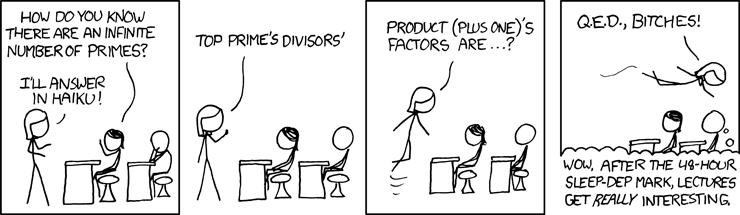
\includegraphics[scale=.5]{comics/622}
\end{center}
